
% drawio link: https://drive.google.com/file/d/1v-PvghSCGyJmhW1MbzjVfO94-1qarLaI/view?usp=sharing

\begin{figure*}[!t]
    \centering
    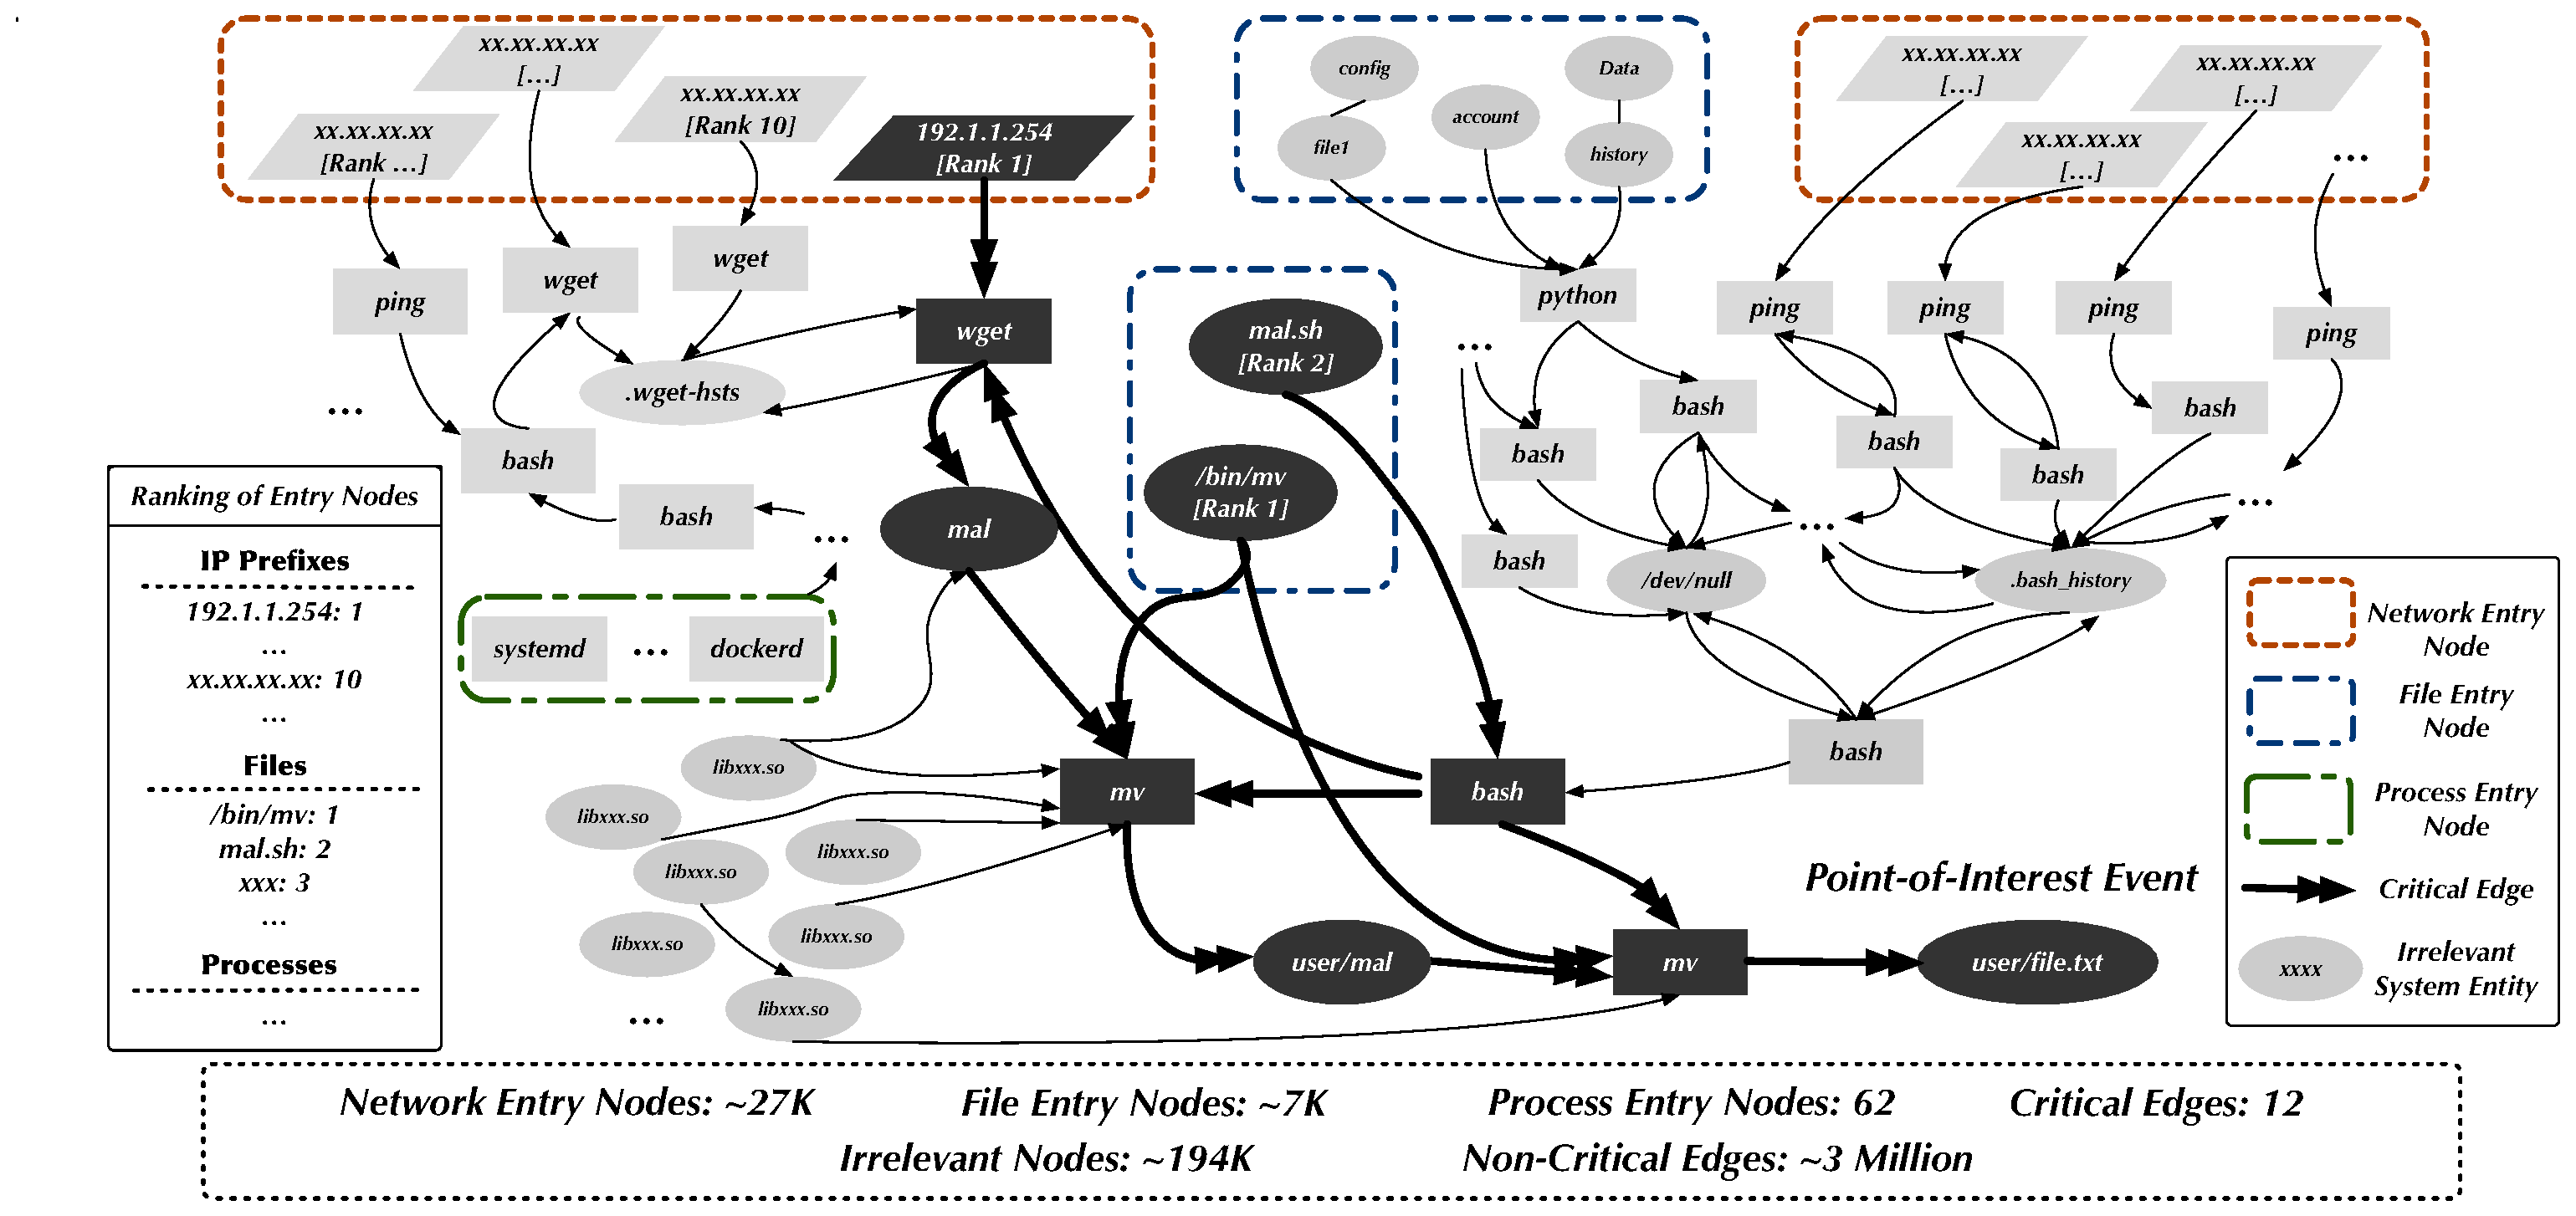
\includegraphics[width=\textwidth, keepaspectratio]{figs/s&p/overview.pdf}
    \caption{Partial dependency graph of an attack that downloads a malicious file and hides the file by renaming it (rectangles for processes, ovals for files, parallelograms for network connections).
    The complete dependency graph constructed from the POI event (renaming to \incode{user/file.txt}) via backward causality analysis contains $194,208$ nodes and $3,273,769$ edges.
    %
    The critical component identified by \tool is colored in dark black, which contains $10$ nodes (including $2$ attack entries) and $12$ edges (these edges are all critical edges).
    As can be seen, \tool significant reduces the size of the dependency graph while preserving the critical attack information.
    }

   % \vspace{2mm}
    \label{fig:motivate}
\end{figure*}


\section{Background and Motivation}

\subsection{System Monitoring}
\label{subsec:system-monitoring}

System monitoring collects auditing events about system calls that are crucial in security analysis, describing the interactions among system entities.
As shown in previous studies~\cite{backtracking,backtracking2,taser,wormlog,gao2018saql,gao2018aiql,mcitracking,logtracking,liu2018priotracker,hassan2019nodoze}, on mainstream operating systems (Windows, Linux, and Mac OS), system entities in most cases are files, processes, and network connections,
and the collected system calls are mapped to three major types of system events:
(1) file access, 
(2) processes creation and destruction, and 
(3) network access. 
Following the established trend, in this work, we consider \emph{system entities} as \emph{files}, \emph{processes}, and \emph{network connections}. 
We consider a \emph{system event} as the interaction between two system entities represented as \emph{$\langle$subject, operation, object$\rangle$}. Subjects are processes originating from software applications (\eg Chrome), and objects can be files, processes, and network connections. 
We categorize system events into three types according to the types of their object entities, namely \emph{file events}, \emph{process events}, and \emph{network events}.


Both entities and events have critical security-related
attributes (\cref{tab:entity-attributes,tab:event-attributes}).
Representative attributes of entities include file name, process executable name, IP, and port.
%unique identifiers to distinguish entities (\eg file path, process name and PID, IP and port).
Representative attributes of events include event origins (\eg start time/end time) and operations (\eg file read/write).
%, and other security-related properties (\eg failure code). 
%(\eg system call return code).

%%%%%%%%%%%%%%%%%%%%%%%%%%
\subsection{Causality Analysis}
\label{subsec:causality-analysis}

Causality analysis~\cite{backtracking,backtracking2,taser,intrusionrecovery,liu2018priotracker,mcitracking,hassan2019nodoze,ma2016protracer} analyzes the auditing events to infer their dependencies 
%among system entities 
and present the dependencies as a directed graph.
%
In the dependency graph $G(E,V)$, a node $v \in V$ represents a process, a file, or a network connection.
An edge $e(u, v) \in E$ indicates a system auditing event that involves two entities $u$ and $v$ (\eg process creation, file read or write, and network access), and its direction (from the source node $u$ to the sink node $v$) indicates the direction of data flow.
Each edge is associated with a time window, $tw(e)$.
We use $ts(e)$ and $te(e)$ to represent the start time and the end time of $e$.
Formally, in the dependency graph, for two events $e_1(u_1, v_1) $ and $e_2(u_2, v_2)$, there exists causal dependency between $e_1$ and $e_2$ if $v_1 = u_2$ and $ts(e_1) < te(e_2)$.

Causality analysis enables two important security applications:
(1) \emph{backward causality analysis} that identifies entry points of attacks, and (2) \emph{forward causality analysis} that investigates ramifications of attacks.
Given a POI event $e_s(u,v)$, a backward causality analysis traces back from the source node $u$ to find all events that have causal dependencies on $u$,
and a forward causality analysis traces forward from the sink node $v$ to find all events on which $v$ has causal dependencies.


\begin{table}[t]
	\centering
	\caption{Representative attributes of system entities}
	\label{tab:entity-attributes}
	\resizebox{0.44\textwidth}{!}{%
		\begin{tabular}{l|l|l}
			\hline
			\textbf{Entity}             & \textbf{Attributes}    & \textbf{Shape in Graph} \\ \hline
			File               & Name, Path          & Ellipse        \\
			Process            & PID, Name, User, Cmd  & Square         \\
			Network Connection & IP, Port, Protocol   & Parallelogram  \\ \hline
		\end{tabular}%
	}
\end{table}


% \eat{
% \begin{table}[!t]
% 	\centering
% 	\caption{Representative attributes of system entities}\label{tab:entity-attributes}
% 	\begin{adjustbox}{0.45\textwidth}
% 		\begin{tabular}{|l|l|}
% 			\hline
% 			\textbf{Entity}		&\textbf{Attributes}\\\hline
% 			File				&Path\\\hline
% 			Process			&PID, Name, User, Cmd\\\hline
% 			Network Connection	& IP, Port, Protocol \\\hline
% 		\end{tabular}
% 	\end{adjustbox}
% 	%	\vspace*{-2ex}

% 	\vspace*{1ex}
% \end{table}
% }
\begin{table}[!t]
	\centering
	\caption{Representative attributes of system events}
	\label{tab:event-attributes}
	\begin{adjustbox}{width=0.44\textwidth}
		\begin{tabular}{l|l}
			\hline
			\textbf{Operation}		& Read/Write, Execute, Start/End\\\hline
			\textbf{Time}		& Start Time/End Time, Duration\\\hline
			\textbf{Misc.}		& Subject ID, Object ID, Data Amount, Failure Code\\\hline
		\end{tabular}
	\end{adjustbox}
	%	\vspace*{-2ex}

	%	\vspace*{1ex}
\end{table}


\eat{
\begin{table}[!t]
	\centering
	\caption{Representative attributes of system events}\label{tab1:event-attributes}
	\begin{adjustbox}{width=0.48\textwidth}
		\begin{tabular}{|l|l|}
			\hline
			Operation		& Read/Write, Execute, Start/End, Rename/Delete.\\\hline
			Time/Sequence		& Start Time/End Time, Event Sequence\\\hline
			Misc.		& Subject ID, Object ID, Failure Code\\\hline
		\end{tabular}
	\end{adjustbox}
	%	\vspace*{-2ex}

		\vspace*{1ex}
\end{table}
}



%%%%%%%%%%%%%%%%%%%%%%%%
\subsection{Motivating Example}
\label{subsec:motivating-example}

\cref{fig:motivate} shows a partial dependency graph of a 
%real 
file hiding activity: 
a suspicious script \incode{mal.sh} is executed to download a malicious file \incode{mal} from a remote host \incode{192.1.1.254}. The file is then moved to \incode {user/mal} and renamed to \incode{user/file.txt}.
%
Given a POI event which renames the file to \incode{user/file.txt}, the dependency graph produced by backward causality analysis 
%from the POI event 
contains $194,208$ nodes and $3,273,769$ edges.
%(the original dependency graph constructed from system audit logs contains $784$ nodes and $6,911$ edges).
The critical edges and attack entries (\incode{192.1.1.254}, \incode{mal.sh}) that represent the attack sequence are colored in dark black.
%
The goal of attack investigation is to inspect the dependency graph to
reveal critical edges and attack entries of the attack.
%obtain the context information (attack entries and critical edges) of the attack.
%the root cause node of the POI, reveal the attack edges, and reconstruct the attack sequence from the massive number of irrelevant nodes and edges.


\myparatight{Challenges}
As observed in \cref{fig:motivate}, attack investigation is a process of \emph{finding a needle in a haystack}: 
a limited number of critical edges (\ie $12$) are buried in an overwhelmingly large number ($\sim 3$ million) of non-critical edges (\ie less-important dependencies),
and same for attack entries (\ie $2$ out of $\sim 35K$ irrelevant entry nodes).
%and normal program execution like Java and Python), 
%and same for the root cause node (\ie $1$) is buried in many other entry nodes (\ie $80$;
%\eg ssh logging in).
%\eg network connections for browser updating and ssh logging in). 
% Existing approaches~\cite{backtracking,backtracking2,taser,intrusionrecovery,liu2018priotracker} require intensive efforts of manually inspecting these edges and nodes for revealing critical edges, identifying root cause nodes, and reconstructing the attack sequence.
% As such, how to automate this process for effectively finding a needle in a haystack becomes a key challenge.



\myparatight{Using \tool to Identify Critical Component}
To remove less-important dependencies introduced by irrelevant system activities, \tool identifies the critical component, a subgraph that consists of mainly 
%relevant dependencies,
critical edges and attack entries,
by (1) computing dependency weights for edges and computing dependency impacts for entry nodes, (2) ranking entry nodes based on their dependency impacts, and (3) performing forward causality analysis from the top-ranked entry nodes to filter out irrelevant parts of the graph.

In this example, we divide the entry nodes into $3$ categories (\ie network connections, files, and processes), and rank the entry nodes in each category.
Here, \tool ranks the IP \incode{192.1.1.254} for \incode{mal} downloading as top $1$, the malicious script \incode{mal.sh} and the executable \incode{/bin/mv}
%for the process \incode{mv}
as top $1$ and top $2$.
By performing forward causality analysis from top-ranked entry nodes and taking the overlap, \tool filters out most of less-important dependencies ($\sim 3$ million) and identifies the critical component (colored in dark black; $10$ nodes, $12$ edges) that preserves all critical edges and attack entries.
